\documentclass{../res/univ-projet}
\usepackage{graphicx}
\usepackage[francais]{babel}
\usepackage[T1]{fontenc}
\usepackage[utf8]{inputenc}
\usepackage{algorithmic}
\usepackage{algorithm}
\usepackage{dsfont}

\graphicspath{{imgHOTP/}}

\title{Authentification à base d'OTP}
\author{D.\bsc{Picard}, A.\bsc{Smondack}, C.\bsc{Hardouin}, J.\bsc{Tayewo}, B.\bsc{Zigh}, G.\bsc{Ferry}, M.\bsc{Michotte} }

\projet{One Time Project}
\projdesc{Étude des systèmes de mots de passe jetables}
\filiere{M1SSI}
\logo{../res/logo_univ.png}



\begin{document}
\maketitle

\begin{abstract}
Ce document présente une analyse de différents systèmes d'OTP tels \og{}OTP\fg{} lui même,\og{}HOTP\fg{}, \og{}TOTP\fg{},
et \og{}OTPW\fg{}. Toutes les informations présentées et analysées proviennent des \href{http://tools.ietf.org/html/rfc2289}{RFC2289} et 
toutes les RFC basées sur celle-ci, soit \href{http://tools.ietf.org/html/rfc4226}{RFC4226}, \href{http://tools.ietf.org/html/rfc4256}{RFC4256}, 
\href{http://tools.ietf.org/html/rfc6238}{RFC6238}, ainsi que de leurs correctifs. Le but de cet article est de déterminer dans quelle mesure 
ces systèmes sont utilisables, sous quelles conditions et avec quelles garanties de sécurité. Ce document réalise également un comparatif entre les 
systèmes précédemment cités.
\end{abstract}

\newpage
\tableofcontents
\newpage
\part{Introduction}
L'authentification permet de vérifier l'identité dont une entité (personne ou machine) se réclame, pour lui autoriser l'accès à des
ressources ou à certains privilèges. La méthode d'authentification la plus connue est celle du login couplé au mot de passe, cependant
ce mécanisme est fragile notamment aux attaques par rejeu, où l'attaquant intercepte un paquet d'identification envoyé par le client et tente de le réutiliser. Ainsi, afin de renforcer la sécurité de cette méthode, 
l'objectif de notre projet est d'étudier les mécanismes d'authentification par mots de passe jetables (OTP) comme second facteur afin de renforcer la sécurité
des méthodes par (login,mot de passe) et de proposer cette fois une méthode d'authentification dite forte.\\
Ce nouveau système fait donc intervenir les OTP. Un OTP (One-Time-Password) satisfait deux critères. Premièrement il n'est pas prévisible ce qui veut dire qu'on ne peut pas prédire 
ou déduire les futurs OTP; deuxièmement un OTP n'est valide que pour une unique session, ce qui veut dire qu'une fois qu'un OTP est utilisé il n'est pas réutilisable, on évite ainsi les
attaques par rejeu.\\
Nous allons donc commencer cet article par une présentation du protocole OTP qui sert de base pour tout les autres protocoles, et dont l'appréhension est donc nécessaire pour la compréhension
de ses protocoles dérivés.
\part{Protocole OTP}
\setcounter{section}{0}
%------------------------------------------------------------------------------
\section{Pré-requis}
  Le système OTP repose principalement sur l'utilisation de fonctions de 
  hachage, les algorithmes les plus courants seront présentés dans ce 
  document.

  OTP est une évolution de S/KEY (système publié par Bellcore), qui est 
  lui-même un système de mot de passe jetable dont la description complète est disponible
  dans la RFC 1760 (datant de 1995).

%------------------------------------------------------------------------------
\section{Généralités}
  Le système OTP (One-Time Password) est un standard décrivant des protocoles 
destinés à la mise en service d'un système d'authentification par mot de passe 
jetable. Ce standard date de 1998.

  Ce système propose une solution de prévention des attaques dites \og par 
rejeu\fg{} (c'est à dire récupérer les login et mot de passe d'une personne pour un 
usage ultérieur). Tout au long de l'étude du système, nous considérerons plusieurs 
entités:

  \begin{description}
    \item[L'utilisateur :] le sujet de l'authentification en vue d'une 
    connexion au serveur;
    \item[Le client :] un logiciel doté d'une interface utilisateur ou un site 
    web permettant une authentification auprès d'un serveur adapté;
    \item[Le serveur :] l'entité qui permet d'authentifier un utilisateur,
    contient une base de données contenant des informations sur l'utilisateur 
    (login, dernier mot de 
    passe utilisé, ...) et dispose d'une routine permettant de vérifier 
    l'authenticité de celui-ci avec le mot de passe jetable qu'il lui a fourni;
    \item[Le token :] élément physique ou logiciel permettant de générer un mot 
    de passe jetable pour un utilisateur;
    \item[Un attaquant :] hacker, malware, etc... Une entité cherchant à 
    usurper 
    l'identité de l'utilisateur vis à vis du serveur en récupérant ses informations 
    de connexion. Ou son accès au service sans ces informations\\
  \end{description}

  Le principe est simple :

  \begin{itemize}
    \item Un utilisateur souhaitant se connecter sur un service via un client
    employant le système OTP dispose d'un token lui permettant de générer un 
    mot de passe jetable 
    (qu'on appellera par la suite otp) que l'interface lui demande;
    \item Le token exécute une série de calculs sur une clé secrète et en tire 
    un otp qu'il communique à l'utilisateur;
    \item l'utilisateur renseigne son login et l'otp au client;
    \item Le client envoie une requête au serveur et lui fournit l'otp; 
    \item Le serveur vérifie le mot de passe en appliquant la fonction de 
    hachage sur celui-ci. Si le résultat correspond au dernier otp utilisé par cet 
    utilisateur, celui-ci est authentifié. Le serveur conserve cet OTP comme dernier
    utilisé\\
  \end{itemize}

  Le mot de passe étant à usage unique, il ne pourra pas servir à un attaquant 
l'ayant récupéré en écoutant les communications entre le client et le serveur.

  Les principaux avantages sont les suivants :

  \begin{itemize}
    \item Le secret n'est jamais transmis entre le client et le serveur.
    \item La sécurité des mots de passe générés repose sur la non-réversibilité 
    de la fonction de hachage utilisée. Ainsi, il est extrêmement difficile (voir 
    impossible) de prédire les prochains mots de passes générés.\\
  \end{itemize}

  Le système OTP fournit ainsi un protection affirmée contre tout type 
  d'attaque contre le vol d'identifiants.
  En revanche elle ne protège pas le client des attaques telles 
  que le vol de sessions\footnote{Vol de cookies.} et l'espionnage.

%------------------------------------------------------------------------------
\section{Approfondissement}
  Nous étudierons ici plus en détail les propriétés du système OTP.

  \subsection{Génération et partage d'un secret}
    Le secret ici est la clé utilisée par le token pour calculer un otp, il 
s'agit d'une phrase de passe généralement fourni en clair par l'utilisateur 
sous forme de données textuelles. 

    À aucun moment cette clé ne doit traverser le réseau, que ce soit lors 
d'une authentification ou d'un changement de clé.

    Ce qui résout la question du partage de la clé. Seul le token connait la 
clé permettant de générer les mots de passe, il est donc impossible à un attaquant 
de la récupérer pour générer lui même les mots de passe (à moins de récupérer 
le token lui-même).

  \subsection{Génération d'un mot de passe jetable}

    La génération d'un otp se déroule en trois étapes :
    \begin{description}
      \item [phase initiale :] combinaison des entrées;
      \item [phase de calcul :] application de la fonction de hachage un 
      certain nombre de fois;
      \item [phase de conversion :] une fonction renvoyant les 64 bits de l'otp 
      sous forme lisible.\\
    \end{description}

    Voyons ces trois étapes en détails.

    \subsubsection{Phase initiale}
      Chaque otp est calculé à partir du \emph{challenge}.

      Le serveur fournit en clair une graine que l'on concatène à la clé. Un 
utilisateur peut donc utiliser la même clé depuis plusieurs machines, le serveur 
enverra des graines différentes. La graine ne doit contenir que des caractères 
alphanumériques et la longueur doit être inférieure à 16. C'est une chaîne de 
caractères sans espace et contenant de préférence des caractères issus du code 
ISO-646. Elle n'est pas sensible à la casse, et on se conformera à la convertir 
en minuscule avant tout calcul.

      La clé et la graine forment ensemble le challenge. La syntaxe du challenge
doit être standard de façon à ce que les générateurs automatisés puissent les 
reconnaitre et en extraire des informations. La syntaxe standard prend la forme 
suivante:
      \begin{center}
          \emph{otp-<algorithmID> <séquence d'entier> <graine>}\\
      \end{center}

      Les trois segments sont séparés par une combinaison de caractères 
d'espacement (espace et/ou tabulation) et doit se terminer de même ou par un 
retour chariot. 

      La chaîne "otp" au début doit être en minuscule.

      L'ID de l'algorithme est sensible à la casse, ceux pré-existants sont en 
      minuscule. Voici ceux utilisés le plus couramment :
      \begin{description}
          \item [MD4] id : md4
          \item [MD5] id : md5
          \item [SHA1] id : sha1 
      \end{description}
      Tout algorithme supplémentaire peut être reconnu en définissant un 
identifiant court.

      La graine suit les mêmes contraintes qu'auparavant : insensible à la 
    casse, convertit en minuscule avant usage.

      Voici un exemple de challenge :
      \begin{center}
          \emph{otp-md5 487 dog2 }\\ 
      \end{center}

      Le challenge est passé à la fonction de hachage puis dans une fonction
      de réduction pour arriver à une taille de 64 bits. Par la suite,
      on notera ce résultat \emph{S}.

    \subsubsection{Phase de calcul}
      Une série d'otp est produite par applications successives de la fonction de 
hachage (un nombre \emph{N} de fois spécifié par l'utilisateur) sur S. Le 
résultat sera le 1\textsuperscript{ier} otp communiqué à l'utilisateur. Le 
suivant sera le résultat de \emph{N-1} occurrences de la fonction de hachage 
sur S. 

      Un espion interceptant la transmission d'un otp ne pourra pas déterminer 
le prochain (l'occurrence \emph{N-2}) car cela impliquerait qu'il ait inversé la 
fonction de hachage. Or c'est sur la non-réversibilité de la fonction de 
hachage choisie que repose la sécurité des otp générés.\\



    \subsubsection{Phase de conversion}
        L'otp généré, fait 64 bits de long. Tout serveur doit être en mesure 
d'accepter un otp sous la forme de 6 mots de 1 à 4 lettres appartenant à la 
norme ISO-646, chaque mot étant choisi dans un dictionnaire de 2048 mots. On compte 
11 bits par mots, pour un total de 66 bits les bits 65 et 66 sont utilisés pour représenter 
une somme de contrôle permettant de valider l'intégrité de l'OTP donné.

        La présentation de l'otp sous la forme de 6 mots doit se faire comme 
suit : en majuscules, et séparés avec un espace. Toutefois, tout serveur 
supportant ce format doit l'accepter sans vérifier la casse ni les séparateurs. 
Le 
premier exemple ci-dessous illustre une sortie de générateur conforme et 
acceptable en entrée. Le second est uniquement acceptable en entrée :
        \begin{center}
            OUST COAT FOAL MUG BEAK TOTE\\
            oust coat foal mug beak tote
        \end{center}

        L'interopérabilité implique que les serveurs et le générateurs 
emploient tous le même dictionnaire. On utilise couramment celui fourni dans la RFC 1760 
(fournit en index D).

        Il est possible de fournir une sortie de générateur en hexadécimal. Le 
serveur doit accepter l'hexadécimal en entrée (sans tenir compte de la casse). 
Les chiffres/lettres peuvent être séparés par des espaces qui seront ignorés 
par le serveur. Voici quelques exemples:
        \begin{itemize}
            \item 3503785b369cda8b              0x3503785b369cda8b
            \item e5cc a1b8 7c13 096b           0xe5cca1b87c13096b
            \item C7 48 90 F4 27 7B A1 CF       0xc74890f4277ba1cf
            \item 47 9 A68 28 4C 9D 0 1BC       0x479a68284c9d01bc
        \end{itemize}

        En plus des formats 6 mots et hexadécimal, le serveur devrait accepter 
l'encodage décrit par le dictionnaire alternatif cité dans les annexes de la RFC. Le répertoire de mots du dictionnaire standard ne doit 
cependant pas être altéré ou oublié. Afin d'éviter toute ambiguïté avec 
l'hexadécimal, on n'emploiera pas les lettre de A à F. Les mots du nouveau dictionnaire sont 
sensibles à la casse et la casse doit être conservée.\\

        Au final, le serveur doit accepter :
        \begin{itemize}
            \item le format 6 mots basé dur les dictionnaires de la RFC1760 et de 
            l'annexe D;
            \item l'hexadécimal;
            \item éventuellement le format 6 mots basé sur le dictionnaire alternatif 
            (cf RFC).
        \end{itemize}
  
  \subsection{Soumission et protocole de vérification}
        Voici ce qui est dit dans la RFC 2289:
    une fois l'OTP transmis au serveur il décodé en une clé de 64 bits puis haché.
    Si ce haché correspond à l'OTP précédent il est donc valide.
    L'utilisateur est authentifié et l'OTP prend la place du précédent.
    
        Seulement un OTP est constitué de 64 bits. selon les fonctions un haché
    d'OTP fait entre 128 et 160 bits. Donc un haché ne pourra jamais correspondre
    à un OTP. La RFC 2289 n'est pas précise sur ce point.
  
  \subsection{Synchronisation}
    Ce système fonctionnant sur un modèle défi/réponse, il est impossible de perdre
    la synchronisation. À chaque fois le serveur demande un OTP bien précis dans la séquence.
  
  \subsection{Réinitialisation}
    Le système étant limité en nombre d'utilisation (génération du $n^{i\grave{e}me}$ 
    hachés lors de l'initialisation) il est nécessaire de réinitialiser le système
    une fois cette limite atteinte sous peine de ne plus pouvoir s'authentifier.
    
    Lors de la ré-initialisation le paramètre seed est renouvelé ce qui permet à
    l'utilisateur de garder la même clé secrète. Soit l'utilisateur spécifie la valeur
    pour seed et le nombre d'OTP à générer soit il utilise la valeur aléatoire suggérée.
    
    La RFC 2289 préconise de permettre à un utilisateur de réinitialiser son système
    à distance sans révéler sa phrase de passe secrète. Ceci n'intervient pas dans
    une implémentation où seul le haché précédent est stocké.

%------------------------------------------------------------------------------
\section{Analyse générale et sécurité}
    \subsection{Avantages et intérêts}
    Les avantages fournis par le système OTP sont ceux fournis par tous les
    systèmes d'authentification à mot de passe jetable. Ce mode de connexion 
    offre donc une résistance aux attaques par rejeu.
    
    Il permet ainsi de s'assurer que la réutilisation de mot de passe par un
    attaquant qui les aurait récupérés lors d'une authentification n'est pas 
    possible.
    
    Ce système peut, de plus, être utilisé conjointement avec un système 
    classique d'authentification par login / mot de passe. On met ainsi en 
    place un système d'authentification dite forte assurant un niveau de 
    sécurité plus important bien que restant moins élevé que les systèmes
    d'authentification cryptographiques.
  
  \subsection{Inconvénients et limites}
  Le protocole d'OTP étudié ici est le premier né des systèmes 
  d'authentification à mot de passe jetable. Ainsi, bien que posant les bases
  de la méthode, il souffre de certains inconvénients d'utilisation. Ces 
  derniers n'engendrent pas de problèmes de sécurité mais empêchent toute 
  utilisation confortable du système.
  
  Parmi ces soucis de confort, le plus remarquable est sans doute le fait
  qu'il n'y a qu'un nombre fixé de connections possibles pour une 
  initialisation donnée. En effet, si lors de l'association du client avec 
  le serveur le nombre de hachés successifs calculés est fixé à 100, seuls 
  99 connexions seront possibles successivement. Une fois cette limite 
  atteinte il sera nécessaire de changer la graine de génération et donc
  de réinitialiser le protocole.
  
  Un autre point important est relatif aux performances de la méthode. En effet
  lorsque le token calcule l'OTP, il doit hacher successivement plusieurs 
  valeurs jusqu'à atteindre le numéro de mot de passe demandé. Or le coup en 
  calcul peut être important pour les premiers OTP demandés.
  
  \subsection{Considérations de sécurité}
    \subsubsection{Attaques exhaustives}
    Les attaques par recherche exhaustive sur le système OTP peuvent être 
    exécutées dans deux buts différents. L'attaquant peut soit chercher à
    trouver la clef secrète de l'utilisateur soit à trouver la valeur de l'OTP
    actuellement demandé.
    
    Dans le premier cas, l'attaquant demande une authentification et récupère 
    le challenge de connexion. Il devra alors calculer la valeur du $N^{ième}$ 
    haché pour toute les valeurs de clef secrète possibles. La résistance aux
    attaques sur ce point dépend donc de la clef de l'utilisateur. Cependant, 
    la longueur de cette clef est limitée inférieurement à 10 caractères. Si
    l'on considère que la clef est codée en ascii 8 bits, on obtient donc une 
    taille minimum de clef de $2^{80}$ bits. Au vu du coup nécessaire au 
    calcul d'un OTP, cette valeur semble raisonnable. De plus, la longueur de 
    la clef peut être étendue jusqu'à plus de 60 caractères augmentant encore
    la résistance.
    
    Dans le second cas, l'attaquant demande un authentification et tente 
    ensuite de trouver la valeur à entrer pour s'authentifier. La méthode est
    simple puisqu'il suffit d'énumérer les valeurs possibles pour un OTP. Dans
    notre cas, l'OTP étant codé sur 64 bits l'attaque s'exécutera en $2^{64}$ 
    opérations. Si l'on considère qu'il est possible d'effectuer $10^9$ 
    tentatives par seconde, alors cette attaque réussit en 58 ans. Le mot de 
    passe étant jetable, ce temps est plus qu'acceptable.
    
    \subsubsection{Attaques par collisions}
        Les collisions recherchées dans cette section sont des collisions dîtes fortes.
    puisqu'il faut trouver un OTP ayant une empreinte bien précise.
    
        Il y a deux façons de voir l'attaque: 
        
        Soit on cherche une collision directe sur
    le prochain OTP auquel cas on applique une fois la fonction de hachage sur $n$ clefs.
    Comme on considère des hachés de 128 à 160 bits cela fait des attaques entre $O(2^128)$
    et $O(2^160)$ ce qui n'est pas envisageable. en cas de réussite cette attaque permet 
    d'obtenir un seul identifiant et donc une seule session.
    
        Soit on génère une suite d'OTP a partir d'une clé choisie jusqu'à trouver
    une collision avec le prochain OTP. Les complexités restent alors les même mais ce type
    d'attaque permettrait d'obtenir plusieurs identifiants et donc plusieurs sessions.
    
    \subsubsection{Failles connues}
      Outre les attaques actives de type espionnage et brute force le système ne possède pas de failles connues.
    
    \subsubsection{Précautions et préconisation}
    La clé doit contenir au moins 10 caractères pour réduire les risques de la 
retrouver par la méthode de recherche exhaustive ou par attaque du dictionnaire. 
Cependant toute implémentation du système OTP doit supporter des clés d'au 
moins 10 à 63 caractères.

    Afin d'assurer l'interchangeabilité des générateurs d'otp, chacun doit 
supporter des clés de 10 à 63 caractères, des clés plus longues sont 
envisageables (mais attention à la compatibilité avec des générateurs plus 
restreints).
  
%------------------------------------------------------------------------------
\section{Utilisations}
  Le protocole ne trouve plus d'utilisation actuellement du fait qu'il existe des protocoles remplissant
  les mêmes fonctions tout en étant plus simples et plus performants. On peut citer par exemple HOTP ou TOTP. Cependant
  cette méthode pourrait quand même être utilisée sans perte de sécurité.
  
%------------------------------------------------------------------------------
\section{Conclusion}
  \subsection{Pérennité du système}
    Le système est obsolète car il a été remplacé par des protocoles plus simples et plus performants.

\part{Protocole HOTP}
\setcounter{section}{0}
\section{Pré-requis}
Le système d'OTP \og{}HOTP\fg{} est un système d'authentification par mot de passe jetable qui étend le système le système OTP définit dans la RFC 2289. Le système OTP 
est étudié plus haut.
Le système HOTP repose principalement sur l'utilisation du mécanisme d'authentification de message HMAC. Ce mécanisme destiné à vérifier si un message n'a pas été altéré
et à authentifier l'expéditeur, repose lui-même sur l'utilisation d'une fonction de hachage et d'un secret partagé. La ou un mécanisme classique de vérification 
d'intégrité de message se contente de hacher ce dernier pour obtenir une empreinte, le mécanisme HMAC utilise une clef secrète pour authentifier l'expéditeur. Cette clef 
est prise en compte de la manière suivante : 
\begin{center}
$HMAC_K(M) = h(K \oplus opad || h(K \oplus ipad || M))$ 
\end{center}
où :\newline
$K$ est la clef secrète \newline
$opad$ = 0x36 répété un certain nombre de fois \newline
$ipad$ = 0x5C répété le même nombre de fois \newline
$\oplus$ est l'opération XOR \newline
$M$ est le message \newline


Dans le cadre de l'authentification de messages, le code HMAC du texte sera envoyé au destinataire sur un canal sécurisé différent de celui utilisé pour la transmission
du message. Le destinataire, une fois le message et le code HMAC reçus, pourra vérifier l'authenticité du message en calculant le code HMAC de ce dernier et en le 
comparant avec celui envoyé.

Le mécanisme HMAC sera ici utilisé pour la génération de mots de passes jetables.

\section{Généralités}
Lors de l'utilisation d'un système de mot de passe jetable le client (ou plus généralement l'entité souhaitant s'authentifier sur le service) fournit au service un 
classique login et un mot de passe. Contrairement aux méthodes classiques d'authentification par login et mot de passe, ici le mot de passe n'est utilisable qu'une seule et 
unique fois et sera donc différent à chaque connexion.
Il existe deux grandes catégories de système de mots de passe jetable : les systèmes dits \og{}synchrones\fg{} et les systèmes dits \og{}asynchrones\fg{}. Les premiers 
reposent sur le partage d'un secret entre le client et le serveur ainsi que sur un élément de synchronisation (i.e un compteur partagé, l'heure actuelle...). Les seconds 
au contraire ne reposent que sur le partage du secret et ne demandent aucune synchronisation entre client et serveur.
Le système \og{}HOTP\fg{} étudié ici est synchrone. Sont principe de fonctionnement est le suivant :
\begin{itemize}
 \item L'utilisateur demande à son token\footnote{Le token est un élément matériel ou logiciel dont la seule fonction est de générer des mots de passe jetables.} de 
 générer un mot de passe jetable.
 \item Le token génère le mot de passe en calculant $HMAC_K(C)$, avec K le secret partagé et C le compteur de synchronisation, puis incrémente le compteur.
 \item L'utilisateur récupère le mot de passe jetable fourni par le token et le passe au serveur d'authentification.
 \item Le serveur calcule la valeur de $HMAC_K(C)$, avec K le secret partagé et le compteur de synchronisation, puis incrémente le compteur.
 \item Si la valeur calculée par le serveur coïncide avec la valeur envoyée par l'utilisateur, ce dernier est authentifié. Dans le cas contraire, il est rejeté
\end{itemize}

Le principal intérêt des méthodes d'authentification par mot de passe jetable, et donc de la méthode HOTP, est d'éviter les attaques dites \og{}par rejeu\fg{} durant 
lesquelles un attaquant récupère le mot de passe durant une communication client-serveur et l'utilise ensuite pour usurper l'identité du client.

\section{Approfondissement}
  Étudions maintenant le fonctionnement précis du système de mot de passe jetable \og{}HOTP\fg{}.
  \subsection{Génération et partage d'un secret}
    Le secret partagé entre le client et le serveur est le point le plus sensible du système d'authentification par mot de passe jetable. En effet, si un attaquant 
    parvient à s'emparer du secret d'un utilisateur, il sera capable de s'authentifier à sa place, mettant en péril la sécurité du compte utilisateur. La méthode 
    \og{}HOTP\fg{} propose pour la génération des secrets deux méthodes : une méthode déterministe et une méthode aléatoire. Détaillons ces deux méthodes.
    
    \subsubsection{Méthode déterministe}
    Pour la méthode déterministe, une clef maitresse, notée $K_M$ doit être enregistrée sur le serveur. Puisque les clefs secrètes de tous les clients seront dérivées 
    de $K_M$, cette clef devra être stockée dans une zone très sécurisée voir inviolable. Lorsque qu'un nouveau client sera ajouté au service de connexion, celui ci
    se verra muni d'une clef secrète, $K_i$, personnelle qui sera partagée avec le serveur. Cette clef sera calculée à partir de la clef $K_M$ et d'une information, $i$, 
    identifiant le client de la manière suivante : \newline
    \begin{center}
     $K_i = h(K_M || i)$ 
    \end{center}
    \hfill{},avec h une fonction de hachage.\newline
    Cette clef constitue un secret unique et robuste si l'on respecte les conditions suivante :
    \begin{itemize}
     \item La fonction $h$ est une fonction de hachage non inversible (md5, SHA\_1...).
     \item Le secret $K_M$ est inviolable.
     \item Le paramètre $i$ est un identifiant unique à chaque utilisateur (ID matériel, numéro de série...)
    \end{itemize}
    
    \subsubsection{Méthode aléatoire}
    Pour la seconde méthode, une clef aléatoire est générée pour chaque nouveau client demandant l'association.
    Afin d'assurer la robustesse du secret, le générateur aléatoire doit être choisi le moins prédictible possible. Il est en général préférable de choisir un générateur 
    matériel, reposant sur l'aléatoire d'un phénomène physique (décomposition de noyaux atomiques, bruit thermique...). A défaut, un très bon générateur pseudo-aléatoire 
    reposant sur l'exécution d'un algorithme (\emph{Yarrow}, \emph{Fortuna}, \emph{Blum Blum Shub}, \emph{ISAAC}...) peut être utilisé. Quel que soit le générateur 
    utilisé, celui ci doit fournir une sortie imprédictible et une distribution de probabilité entre les clefs aussi uniforme que possible.
  
  Quelle que soit la méthode de génération utilisée, la clef produite doit être d'une longueur correspondant aux standards de sécurité actuels. A l'heure ou ce rapport 
  est écrit, une longueur de clef de 128 bits parait être un minimum. Choisir une longueur supérieure ou égale à 160 bits semble plus raisonnable et une clef de 256 
  bits ou plus fournit un très bon niveau de sécurité.
    
  \subsection{Génération d'un mot de passe jetable}
  La génération d'un OTP avec la méthode HOTP repose sur l'utilisation d'un compteur incrémental et de la clef secrète, tous deux partagés entre le token et le service de 
  validation. Une fonction HMAC définie pour une fonction de hachage donnée est aussi utilisée pour produire la base de l'OTP.
  Au global, la génération de l'OTP se décompose en trois étapes principales selon l'algorithme \ref{HOTP:gene}.
  \begin{algorithm}
  \caption{Génération d'un OTP par HOTP}
    \label{HOTP:gene}
   
    \begin{algorithmic}
    \REQUIRE $K$ une clef secrète, $C$ un compteur de synchronisation.
    \STATE $HVal \leftarrow HMAC(K, C)$
    \STATE $HVal \leftarrow tronc(HVal)$
    \STATE $HVal \leftarrow binToDec(HVal)$
    \STATE $C \leftarrow C + 1$
    \newline
    \RETURN $HVal \bmod 10^L$ // L : longueur souhaitée de l'OTP
    \end{algorithmic}
  \end{algorithm}
  
  Dans ce schéma, la première étape consiste à calculer la valeur de HMAC pour la clé secrète partagée et en prenant pour message le compteur de synchronisation. La 
  longueur de la valeur obtenue dépend de la fonction de hachage utilisée. On aura par exemple une chaine de 160 bits en utilisant la fonction SHA\_1.
  On pourrait utiliser la sortie de la fonction HMAC comme OTP cependant, écrite en décimal cette valeur se représenterait sur 48 chiffres et serait peut pratique à entrer 
  pour un utilisateur. C'est pourquoi les étapes 2 et 3 vont permettre de réduire la longueur de l'OTP à une valeur sur 10 chiffres via les fonctions $tronc$ et 
  $binToDec$. La fonction $tronc$, qui extrait une chaine de 31 bits de la sortie de $HMAC$, est définie par l'algorithme \ref{HOTP:trunc}.
  
  \begin{algorithm}
    \caption{tronc : Réduction de la sortie de $HMAC$}
    \label{HOTP:trunc}
    
    \begin{algorithmic}
      \REQUIRE S une chaine de bit
      \ENSURE S est de longueur 31 bits
      \STATE $offBits \leftarrow$ Les 4 bits de poids faible de S[19]
      \STATE $offset \leftarrow binToDec(offBits)$ // 0 $\leq offset \leq$ 15
      \STATE $P \leftarrow S[offset]..S[offset + 3]$ \newline
      \RETURN Les 31 derniers bits de $P$
    \end{algorithmic}
  \end{algorithm}

  La fonction $binToDec$, quant à elle, va convertir la chaine binaire retournée par $tronc$ en un nombre décimal, composé de 10 chiffres. Afin de faciliter encore un peu 
  plus la saisie du mot de passe jetable, on ne conservera qu'une partie du nombre à 10 chiffres en en prenant le modulo $10^P$, o\`u P est la longueur souhaitée de l'OTP.
  Afin que le mot de passe soit à la fois facilement utilisable et sécurisé, il est conseillé de choisir une valeur de $P$ comprise entre 6 et 8 inclus.
  Après la génération du mot de passe, le compteur de synchronisation est incrémenté pour garantir l'unicité de la valeur produite.
  
  \subsection{Soumission et protocole de vérification}
  La soumission du mot de passe jetable est, pour HOTP, indépendante du reste du système. Dans la majorité des cas, cette étape passera par l'utilisation d'une interface 
  de connexion graphique ou en ligne de commande. Nous nous intéresserons dans cette section à la partie vérification du mot de passe par le serveur. Cette étape est 
  décrite dans l'algorithme \ref{HOTP:verif}.  
  \begin{algorithm}
    \caption{Vérification d'un mot de passe jetable.}
    \label{HOTP:verif}
    
    \begin{algorithmic}
      \STATE $attentNB \leftarrow 0$
      \STATE $C \leftarrow$ compteur de synchronisation de l'utilisateur
      \STATE $K \leftarrow$ clef secrète de l'utilisateur
      \STATE $OTP_1 \leftarrow HOTP_K(C)$
      \WHILE{$attentNB < MAX\_ATTENT$}
	\STATE $OTP_2 \leftarrow$ récupérer\_OTP
	\STATE $attentNB \leftarrow attentNB + 1$
	\IF{$OTP_1 = OTP_2$}
	  \STATE $C \leftarrow C + 1$
	  \STATE accepter l'utilisateur
	\ELSE
	  \IF{resynchro possible}
	    \STATE $resynchro$
	    \STATE accepter l'utilisateur
	  \ENDIF
	\ENDIF
      \ENDWHILE
      \STATE $verouiller$
      \STATE $prevenir$
    \end{algorithmic}
  \end{algorithm}
  
  Dans cet algorithme, la variable $attentNB$ représente le nombre de tentatives d'OTP déjà effectuées par l'utilisateur. Elle permet de contrôler le nombre maximal de mots 
  de passes entrés entre deux authentification réussies dans le but d'éviter les attaque par \emph{brute force}.
  L'algorithme nécessite aussi de connaitre la clef secrète et le compteur de synchronisation liés à l'utilisateur. Le mode de récupération de ces informations n'est pas 
  détaillé dans cet algorithme puisqu'il est complètement indépendant de la méthode HOTP. Dans la majorité des cas, ces informations seront stockées dans une base de 
  données et la récupération se résumera donc à une requête sur cette dernière. Il n'est pas possible de se passer de ces deux informations puisque le serveur 
  d'authentification doit être capable de calculer la valeur de $HOTP_K(C)$ de la même manière que le token de l'utilisateur afin de vérifier l'exactitude la valeur 
  reçue.
  
  Dans sa généralité, l'algorithme de vérification ressemble fortement à un algorithme d'authentification par login / mot de passe standard. A savoir, on demande à 
  l'utilisateur de fournir ses paramètres de connexion et on les vérifie. Si les données passées s'avèrent correctes, l'utilisateur est authentifié, sinon on recommence 
  l'opération jusqu'à l'obtention de données correctes ou jusqu'à atteindre le nombre maximal de tentative. Cependant, on retrouve une différence dans l'appel aux 
  fonctions \og{}resynchro possible\fg{} et \og{}resynchro\fg{}. Ces fonctions, détaillées dans la section \ref{HOTP:synchro}, on pour but d'assurer la cohérence du 
  compteur de synchronisation partagé.
  
  \subsection{Synchronisation}
  \label{HOTP:synchro}
  Par nature, le système HOTP requière que les compteurs du serveur et du token soient synchronisés. En effet, dans le cas contraire, les valeurs de l'OTP calculées par le 
  token et le service d'authentification seraient différentes et aucun utilisateur ne pourrait se connecter.  Si le serveur incrémente le compteur de synchronisation à 
  chaque connexion réussie, le token l'incrémente lui à chaque génération et il est donc aisé de perdre la synchronisation entre le client et le token.
  
  Les fonctions \og{}resynchro possible\fg{} et \og{}resynchro\fg{} présentes dans l'algorithme \ref{HOTP:verif} ont pour fonction d'assurer que les écarts de 
  synchronisations n'empêcheront pas la connexion de l'utilisateur. Leur principe est simple et consiste à comparer la valeur donnée par l'utilisateur avec plusieurs 
  valeurs d'OTP successives proches de la valeur théorique. Par exemple, si l'OTP fourni par l'utilisateur ne correspond pas à $HOTP_K(C)$ alors on vérifiera si il 
  correspond à $HOTP_K(C + 1)$ et ainsi de suite jusqu'à trouver une valeur correspondant ou dépassant le nombre de valeur vérifiables autorisées. Les algorithmes 
  correspondant aux deux fonction de synchronisation sont les algorithmes \ref{HOTP:isSynch} et \ref{HOTP:synch}.

  \begin{algorithm}
    \caption{Vérification de la possibilité de resynchronisation}
    \label{HOTP:isSynch}
    
    \begin{algorithmic}
      \REQUIRE $OTP$ la valeur de l'OTP fournie par l'utilisateur
      \REQUIRE $K$ la clef secrète de l'utilisation
      \REQUIRE $C$ la valeur du compteur de synchronisation pour le token
      \STATE $MAX\_FWD \leftarrow a$ //$MAX\_FWD$ contient le nombre maximal de valeurs a vérifier
      \FOR{$i$ de $1$ à $MAX\_FWD$}
	\STATE $OTP2 \leftarrow HOTP_K(C + i)$
	\IF{$OTP = OTP2$}
	  \RETURN vrai
	\ENDIF
      \ENDFOR
      \RETURN faux
    \end{algorithmic}
  \end{algorithm}
  
  \begin{algorithm}
    \caption{Resynchronisation}
    \label{HOTP:synch}
    
    \begin{algorithmic}
      \REQUIRE $OTP$ la valeur de l'OTP fournie par l'utilisateur
      \REQUIRE $K$ la clef secrète de l'utilisation
      \REQUIRE $C$ la valeur du compteur de synchronisation pour le token
      \STATE $MAX\_FWD \leftarrow a$ //$MAX\_FWD$ contient le nombre maximal de valeurs a vérifier
      \FOR{$i$ de $1$ à $MAX\_FWD$}
	\STATE $OTP2 \leftarrow HOTP_K(C + i)$
	\IF{$OTP = OTP2$}
	  \STATE $C \leftarrow C + i + 1$
	  \STATE accepter l'utilisateur
	\ENDIF
      \ENDFOR
      \STATE rejeter l'utilisateur
    \end{algorithmic}
  \end{algorithm}
  
  Les deux algorithmes sont très similaires. Le premier parcoure les valeurs autorisées à la recherche d'une concordance, le deuxième parcours à son tour les valeurs pour 
  mettre à jour la valeur du compteur du serveur. En pratique, ces deux algorithmes pourront être fusionnés en un seul vérifiant la possibilité de synchronisation et 
  effectuant cette dernière à la suite.
  
\section{Analyse générale et sécurité}

  \subsection{Avantages et intérêts}
  L'avantage principal du protocole \og{}HOTP\fg{} vient du fait qu'il est parmi les méthodes d'OTP les plus utilisées. Ainsi, des \emph{tokens} basés sur cette méthode 
  seront compatibles avec un grand nombre de services d'authentification existants. En particulier, la majorité des tokens compatibles avec la norme OATH (Initiative For 
  Open Authentication) se conforment à la spécification RFC-4226 et reposent donc sur HOTP.
  
  \subsection{Considérations de sécurité}
  L'étude menée sur la sécurité de l'algorithme HOTP est résumée dans cette section.
  Cette analyse est réalisée dans le cas ou $Digit = 6$, avec $Digit$ le nombre de chiffres composant l'OTP, ce qui est le strict minimum 
  recommandé dans ce document.\\
  Soient :
  \begin{itemize}
   \item S la taille de la fenêtre de synchronisation.
   \item V nombre de tentatives autorisées.
   \item Digit le nombre de chiffres composant le mot de passe jetable.
   \item K une clé secrète de l'utilisateur.
   \item C le compteur de synchronisation partagé.
  \end{itemize}

    \subsubsection{Attaques exhaustives}
    Le mot de passe jetable est généré grâce à l'algorithme SHA-1. Cet algorithme est réputé pour fournir une sortie quasi aléatoire donnant une distribution 
    de probabilité quasi uniforme. Ainsi, on peut supposer raisonnablement que la probabilité $\mathds{P}(H = $HMAC-SHA-1$(K, C)) = \frac{1}{2^{160}}$. 
    Après passage par la fonction troncature, la sortie de la fonction HMAC est réduite à une taille de Digit chiffre. On a donc $10^{Digit}$ valeurs de sortie 
    possibles qui, si l'on considère que la fonction de troncature ne change pas la distribution de probabilité, sortent avec une probabilité équitable de
    $\mathds{P}(OTP = HOTP(K, C)) = \frac{1}{10^{Digit}}$. 
    
    Or, le serveur en utilisant les fonctions de synchronisation, permet à un utilisateur de tester jusqu'à $s$ valeurs simultanément, où s est la taille de 
    la fenêtre de resynchronisation. De plus, il autorise aussi un utilisateur à effectuer jusqu'à v tentatives de connexion successives. Ceci augmente donc 
    la probabilité de réussite d'un utilisateur par un facteur $s \times v$.
    
    On obtient finalement la probabilité de réussite d'un attaquant par brute force, $P_{finale} = \frac{sv}{10^{Digit}}$.
   
    Supposons que le nombre de requêtes de vérification, $v$, est au plus 3.
    Avec $Digit = 6$, $s = 3$. On obtient : probabilité de réussite, $P =  \frac{3 \times 3}{10^6} = 9 \times 10^{-6}$
    
    Bien entendu, cette probabilité peut être augmentée ou diminuée en faisant varier la taille de la sortie de la fonction de troncature. Il faut cependant
    garder en tête que cette valeur doit rester inférieure à 10 et idéalement à 8 pour garder la simplicité d'utilisation.
    
    \subsubsection{Attaques par collisions}
    Les attaques par collisions concernent notamment les attaques sur SHA-1. Une collision pour une fonction de hachage h est la donnée d'une paire x, y telle 
    que $x \neq y \wedge H(x) = H(y)$.\\
    Pour SHA-1 avec 160 bits, l'attaque utilisant le paradoxe des anniversaires trouve une collision en $2^{80}$ essais. On a longtemps pensé que c'était 
    la meilleure attaque possible jusqu'à ce que Wang, Yin et Yu annoncent le 15 Février 2005, l'existence d'une attaque trouvant une collision en 
    $2^{69}$ essais. La meilleure attaque à ce jour s'exécute avec une complexité de $2^{61}$, cependant, aucune vraie collision n'a encore été trouvée.
    
    Quoiqu'il en soit, la faiblesse de SHA-1 en ce qui concerne les collisions ne se propage pas à la fonction HMAC. Cela est dû à l'utilisation de la clef secrète
    qui, agissant comme un sel, rend la recherche de collision bien moins aisée.
    
    \subsubsection{Failles connues}
    Le protocole HOTP ne possède aucune faille connue mis à part les failles héritées de OTP.
    En particulier il est sensible aux \og race attacks \fg{} et aux attaques de type \og man in the middle \fg{} qui sont aussi valables sur une  authentification faible, 
    
    \subsubsection{Précautions et préconisation}
    Il est conseillé de choisir une longueur d'OTP entre 6 et 8 caractères afin que le mot de passe soit à la fois facilement utilisable et sécurisé.
    Un tunnel SSH est fortement recommandé afin d'éviter les attaques par \og race attacks \fg{} et \og man in the middle \fg{}.
    La taille de la fenêtre de resynchronisation devrait être fixé entre 3 et 5 afin de pouvoir à la fois être pratique pour l'utilisateur et assez résistant
    à une attaque par brute force.
    
\section{Utilisations}
Les utilisations pour l'implantation du protocole HOTP sont variées, on peut très bien s'en servir à des fins personnelles, pour sécuriser ses données ou 
dans un domaine professionnel.
  \subsection{Cas concrets d'utilisation}
  Google Authenticator
  \begin{itemize}
    \item Google Authenticator est un logiciel open-source qui est basé sur une authentification en deux étapes. Celui-ci est implémenté sur différentes plateformes 
	  mobiles comme iOS, Android, Blackberry, et il est aussi adaptable sur les modules PAM
	  \begin{figure}[h!]
	    \centerline{\includegraphics[scale=0.45]{GoogleAuthenticator_2.jpg}}
	    \caption{Google Authenticator}
	  \end{figure}  
  \end{itemize}
  \newpage
  OATH (Initiative for Open Authentication) Toolkit
  \begin{itemize}
    \item OATH Toolkit fournit une suite de composant pour la construction de systèmes d'authentification par mots de passe jetable. 
	  Les composant comprennent une librairie de programmation en C, un outil en lignes de commandes pour la génération et la validation d'OTP, et un PAM.
  \end{itemize}
  
  LinOTP
  \begin{itemize}
    \item LinOTP est une solution basée Linux pour gérer des systèmes d'authentifications à deux facteurs avec mots de passe jetables.
	  Il est implémenté comme un service web basé sur le framework python. C'est le seul serveur d'authentification open-source certifié par OATH.
	  \begin{figure}[h!]
	    \centerline{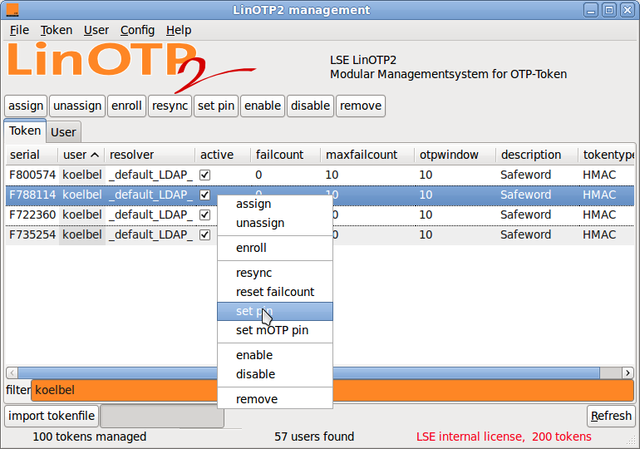
\includegraphics[scale=0.4]{linOTP.png}}
	  \end{figure}
  \end{itemize}  
  
  \subsection{Pérennité du système}
    Comme nous avons pu le voir, le système HOTP ne possède pas de faille de sécurité référencée. De plus, le système n'est pas affecté par les faiblesses des fonctions de 
    hachage, notamment au niveau des collisions. Ainsi, il est fortement envisageable que la fonction HMAC\_SHA\_1 puisse être utilisée pour générer des OTP pour une durée
    encore importante sans compromettre sa sécurité.
    
    De plus, si la fonction HMAC\_SHA\_1 se trouve dépréciée dans le futur, il suffirait de la remplacer par une nouvelle version reposant sur une fonction de hachage plus 
    forte telle que keccak ou whirlpool. Ce qui ne nécessiterait que peu de mises à jour.
    
    On peut donc considérer ce système de calcul d'OTP comme pérenne.
    
\part{Protocole TOTP}

\setcounter{section}{0}
\section{Pré-requis}
Le système d'authentification par mot de passe jetable \og{}TOTP\fg est une extension du système \og{}HOTP\fg{}, par conséquent, il repose sur les mêmes concepts. Ces 
derniers ayant déjà été donnés dans le document relatif à \og{}HOTP\fg{}, nous ne les détaillerons pas de nouveau ici.

\section{Généralités}
Le principe général de fonctionnement du système \og{}TOTP\fg{} est strictement identique à celui du système \og{}HOTP\fg{} à une différence près. Ici, un paramètre 
temporel est utilisé en lieu et place du compteur de synchronisation. Ainsi, la fonction $HMAC_K$ utilisée par \og{}HOTP\fg{} ne sera plus appelée avec pour paramètre la 
valeur du compteur de synchronisation mais avec la valeur $T = \lfloor{}\frac{curTime - T_0}{X}\rfloor{}$, où $curTime$ représente le temps Unix actuel, $T_0$ le temps Unix \og{}
d'origine\fg{} et $X$ un quantum de temps arbitraire.

\section{Approfondissement}
  \subsection{Génération et partage d'un secret}
    Le problème de génération et de partage de secret pour \og{}TOTP\fg{} est strictement identique à celui de \og{}HOTP\fg{} reportez vous au document relatif à ce 
    dernier pour un détails de méthodes.
    
  \subsection{Génération d'un mot de passe jetable}
    La génération des mots de passe jetables pour le système \og{}TOTP\fg{} est similaire à celle de \og{}HOTP\fg{} hormis sur le point du calcul de $HMAC$. En somme, la 
    génération peut être décrite par l'algorithme \ref{TOTP:gene}.
    \begin{algorithm}
      \caption{Génération d'un OTP par TOTP}
      \label{TOTP:gene}
   
      \begin{algorithmic}
	\REQUIRE $K$ une clef secrète
	\STATE $T \leftarrow \lfloor{}\frac{curTime - T_0}{X}\rfloor{}$
	\STATE $HVal \leftarrow HMAC(K, C)$
	\STATE $HVal \leftarrow tronc(HVal)$
	\STATE $HVal \leftarrow binToDec(HVal)$
	\newline
	\RETURN $HVal \bmod 10^L$ // L : longueur souhaitée de l'OTP
      \end{algorithmic}
    \end{algorithm}
    
    Les fonctions $tronc$ et $binToDec$ utilisées dans l'algorithme \ref{TOTP:gene} sont strictement identiques à celle utilisée dans l'algorithme de génération de 
    \og{}HOTP\fg{}. Référez vous au document traitant de \og{}HOTP\fg{} pour plus de détails.
    
  \subsection{Soumission et protocole de vérification}
    La vérification de mot de passe jetable suis le même schéma général que pour le système \og{}HOTP\fg{}. On trouve cependant quelque détails différents. Ces derniers 
    sont résumés dans l'algorithme \ref{TOTP:verif}.
    \begin{algorithm}
      \caption{Vérification d'un mot de passe jetable.}
      \label{TOTP:verif}
      
      \begin{algorithmic}
	\STATE $attentNB \leftarrow 0$
	\STATE $T \leftarrow \lfloor{}\frac{curTime - T_0 + \Delta_t}{X}\rfloor{}$
	\STATE $K \leftarrow$ clef secrète de l'utilisateur
	\STATE $OTP_1 \leftarrow TOTP_K(C)$
	\WHILE{$attentNB < MAX\_ATTENT$}
	  \STATE $OTP_2 \leftarrow$ récupérer\_OTP
	  \STATE $attentNB \leftarrow attentNB + 1$
	  \IF{$OTP_1 = OTP_2$}
	    \STATE accepter l'utilisateur
	  \ELSE
	    \IF{resynchro possible}
	      \STATE $resynchro$
	      \STATE accepter l'utilisateur
	    \ENDIF
	  \ENDIF
	\ENDWHILE
	\STATE $verouiller$
	\STATE $prevenir$
      \end{algorithmic}
    \end{algorithm}
    Ainsi, on retrouve bien le schéma général de vérification vu précédemment, utilisant la valeur $T$ décrite plus haut au lieu de celle du compteur de synchronisation.
    Cependant, dans cet algorithme, la valeur de $T$ est légèrement altérée afin d'y faire apparaitre la valeur $\Delta_t$. Cette dernière est utilisée pour garantir la 
    synchronisation temporelle entre le client et le serveur. Le fonctionnement et le calcul de cette valeur sont décrits dans la section \ref{OTP:syncSec}.
    
  \subsection{Synchronisation}
  \label{OTP:syncSec}
    De même que pour le système \og{}HOTP\fg{}, il est possible que le serveur et le client perdent leur synchronisation temporelle. Il suffit pour cela que
    l'horloge du client ou celle du serveur soit plus rapide que son homologue. Bien que l'utilisation de plus en plus répandue des serveur de synchronisation 
    temporelle mondiaux tende à réduire les possibilités de décalage des horloge, ce cas reste à envisager. C'est pourquoi on retrouve les fonction \og{}resynchro 
    possible\fg{} et $resynchro$, chargées d'assurer la cohérence des vérification d'OTP en cas de désynchronisation d'horloge. Les descriptions de ces fonctions sont 
    données dans les algorithme \ref{TOTP:isSynch} et \ref{TOTP:synch}.
    \begin{algorithm}
      \caption{Vérification de la possibilité de resynchronisation}
      \label{TOTP:isSynch}
      
      \begin{algorithmic}
	\REQUIRE $OTP$ la valeur de l'OTP fournie par l'utilisateur
	\REQUIRE $K$ la clef secrète de l'utilisation
	\STATE $T \leftarrow \lfloor{}\frac{curTime - T_0 + \Delta_t}{X}\rfloor{}$
	\STATE $MAX\_BWD \leftarrow b$ //$MAX\_BWD$ contient le nombre maximal de valeurs a vérifier vers l'arrière
	\STATE $MAX\_FWD \leftarrow a$ //$MAX\_FWD$ contient le nombre maximal de valeurs a vérifier vers l'avant
	\FOR{$i$ de $-MAX\_BWD$ à $MAX\_FWD$}
	  \STATE $OTP2 \leftarrow HOTP_K(T + i)$
	  \IF{$OTP = OTP2 AND not\_used(OTP)$}
	    \RETURN vrai
	  \ENDIF
	\ENDFOR
	\RETURN faux
      \end{algorithmic}
    \end{algorithm}
    
    \begin{algorithm}
      \caption{Resynchronisation}
      \label{TOTP:synch}
      
      \begin{algorithmic}
	\REQUIRE $OTP$ la valeur de l'OTP fournie par l'utilisateur
	\REQUIRE $K$ la clef secrète de l'utilisation
	\STATE $T \leftarrow \lfloor{}\frac{curTime - T_0 + \Delta_t}{X}\rfloor{}$
	\STATE $MAX\_BWD \leftarrow b$ //$MAX\_BWD$ contient le nombre maximal de valeurs a vérifier vers l'arrière
	\STATE $MAX\_FWD \leftarrow a$ //$MAX\_FWD$ contient le nombre maximal de valeurs a vérifier vers l'avant
	\FOR{$i$ de $-MAX\_BWD$ à $MAX\_FWD$}
	  \STATE $OTP2 \leftarrow HOTP_K(T + i)$
	  \IF{$OTP = OTP2 AND not\_used(OTP)$}
	    \STATE $\Delta_t \leftarrow \Delta_t + i * X$
	    \STATE accepter l'utilisateur
	  \ENDIF
	\ENDFOR
	\STATE rejeter l'utilisateur
      \end{algorithmic}
    \end{algorithm}
    
    Le fonctionnement de ces algorithmes est simple. Il s'agit de rechercher dans une fenêtre temporelle donnée une valeur d'OTP correspondant à celle donnée par 
    l'utilisateur. Si une telle valeur est trouvée, on calcule le décalage temporel entre les deux parties et on l'ajoute à la valeur courante du décalage $\Delta_t$.
    Sinon, l'utilisateur est rejeté.
    Comme pour le système \og{}HOTP\fg{}, ces deux fonctions pourront, en pratique, être fusionnées en une seule réalisant à la fois la vérification et la 
    synchronisation.
  
\section{Analyse générale et sécurité}
Analysons maintenant cette méthode et sa sécurité.

  \subsection{Avantages et intérêts}
  Le système \og{}TOTP\fg{} est une extension du système \og{}HOTP\fg{}. Par conséquent, il en reprend les principaux avantages. De plus, grâce à l'utilisation du temps 
  à la place d'un compteur de synchronisation, la synchronisation de ce système est plus difficile à perdre. En effet, lors de l'utilisation de \og{}HOTP\fg{}, il suffit 
  que l'utilisateur demande au \emph{token} plusieurs mots de passes de suite sans les utiliser pour perdre la synchronisation des parties. Pour \og{}TOTP\fg{}, le seul 
  moyen de perdre la synchronisation est que les horloges du client et du serveur n'avancent pas à la même vitesse. Hors, pour que la synchronisation soit décalée d'une 
  \og{}case\fg{}, il faut que le décalage d'horloge soit supérieur à $X$, qui , s'il est correctement choisi, doit être de l'ordre de quelques dizaines de seconde
  ce qui est considérable pour un décalage d'horloge. Bien entendu, il faut que les horloges du client et du serveur aient été synchronisées une première fois lors de 
  la première connexion ou lors de l'inscription de l'utilisateur sur le service.
  
  \subsection{Considérations de sécurité}
  La sécurité du protocole TOTP est directement héritée de celle de son parent HOTP. Ainsi, les probabilités de réussite des attaques exhaustives et les sensibilités au attaques 
  par collisions sont strictement identique modulo les valeurs choisies pour les tailles de fenêtre de resynchronisation et de nombre de tentatives autorisées.
  
    \subsubsection{Précautions et préconisation}
    En général, les précautions à prendre lors de l'utilisation de TOTP sont les mêmes que celles à prendre pour HOTP. Cependant, la taille de la fenêtre de resynchronisation
    doit être revue. En effet, lors de l'utilisation de TOTP, il est possible que le client soit décalé temporellement par rapport au serveur ou le contraire. De ce fait
    lors de la resynchronisation, le serveur doit confronter l'OTP non seulement avec les prochaines valeurs possibles mais aussi avec les précédentes. Aussi, pour éviter qu'un
    utilisateur puisse se connecter plusieurs fois avec le même mot de passe, il est nécessaire de conserver une liste des derniers OTP utilisés. Lors de la resynchronisation, 
    les valeurs de l'OTP données seront confrontées avec celles de la liste pour valider l'utilisation unique. La liste devra retenir au moins autant de mots de passes utilisés que 
    la taille de la fenêtre de resynchronisation vers l'arrière + 1.
    
    Au final, il sera raisonnable de fixer la taille de la fenêtre afin de permettre la validation à deux fenêtres vers l'arrière pour trois vers l'avant.
    
\section{Utilisations}
Tout comme HOTP, les utilisations pour l'implantation du protocole TOTP sont variées, on peut très bien s'en servir à des fins personnelles, pour sécuriser ses données ou 
dans un domaine professionnel.
  \subsection{Cas concrets d'utilisation}
  \begin{description}
   \item \textbf{Utilisation côté serveur}
   \begin{description}
    \item - Google avec son Google Autentificator
    \item - Amazon supporte également TOTP qui peut être utilisé avec les clients suivants: AWS (Multi-Factor Authentication) Amazon Virtual MFA ou le Google Authenticator.
    \item - DropBox
    \item - LastPass
    \item - GitHub
    \item - LinOTP
    \item - multiOTP
   \end{description}

   \item \textbf{Utilisation côté client}
   \begin{description}
    \item - Google Authenticator est un logiciel open-source qui est basé sur une authentification en deux étapes. Celui-ci est implémenté sur différentes plateformes 
	  mobiles comme iOS, Android, Blackberry, et il est aussi adaptable sur les modules PAM
	  \begin{figure}[h!]
	    \centerline{\includegraphics[scale=0.45]{imgHOTP/GoogleAuthenticator_2.jpg}}
	    \caption{Google Authenticator}
	  \end{figure}  
    \item - OATH Toolkit OATH Toolkit fournit une suite de composant pour la construction de systèmes d'authentification par mots de passe jetable. 
	  Les composant comprennent une librairie de programmation en C, un outil en lignes de commandes pour la génération et la validation d'OTP, et un PAM.
    \item - Microsoft's Authenticator est un logiciel pour les Windows Phone
    \item - Red Hat's FreeOT est un logiciel pour Android et iOS.
   \end{description}
  \end{description}
  
\section{Conclusion}
  \subsection{Pérénité du système}
   La pérennité du système TOTP est au moins aussi importante que celle de HOTP.

\part{Protocole OTPW}
\setcounter{section}{0}
\section{Pré-requis}
        Le générateur d'OTP repose sur la fonction de hachage RipeMD-160. Tant pour
    la génération de hachés et la vérification par comparaison de hachés
    que pour générer de l'entropie.

        Ce protocole requiert pour pouvoir fonctionner de pouvoir stocker
    sur le serveur un fichier contenant la liste de vérification des OTP (environ 
    4ko pour 300 OTP) dans le dossier de l'utilisateur sous le nom \verb?.otpw?
    
        L'utilisateur quant à lui est supposé pouvoir garder une liste de chaînes
    de caractères nécessaire à la création des OTP. Cette liste est habituellement
    imprimée sur une feuille de papier.

\section{Généralités}
        Ce protocole fonctionne grâce à deux listes numérotées, une permettant 
    de former les OTP. Et une permettant de vérifier les OTP. Afin d'initialiser
    ces listes l'utilisateur doit entrer un mot de passe que l'on appellera plus
    tard le préfixe. 
    
        Le serveur va générer deux listes: une qu'il va donner à l'utilisateur que
    l'on appellera liste de suffixes, et une qu'il va garder et qui permettra de
    vérifier les OTP.

        Ces OTP sont construits en concaténant le préfixe avec l'un des suffixes.
    Le serveur va hacher l'OTP avec la fonction RipeMD-160 ce haché et le comparer
    avec celui de sa liste afin de vérifier sa validité.

        Quand un utilisateur veut s'authentifier le client demande un challenge 
    au serveur. Ce challenge est un numéro permettant d'identifier un suffixe sur
    la liste. L'utilisateur devra rentrer son login ainsi que l'OTP généré avec
    ce suffixe. Le serveur authentifiera l'utilisateur si l'OTP correspond bien 
    a celui ayant le même numéro dans sa liste. Si l'utilisateur est authentifié
    alors il rayera de sa liste le haché de l'OTP.

\section{Approfondissement}
\subsection{Génération et partage d'un secret}
        La génération de secret ne se fait qu'en ayant accès au serveur. Une fois
    connecté sur le serveur l'utilisateur doit exécuter la commande \verb?otpw-gen?.
    Cette commande demandera à l'utilisateur de rentrer son mot de passe préfixe.

        Une fois le mot de passe rentré le serveur initialisera les deux listes avec 
    l'algorithme suivant.
    %TODO: Envisager une version de l'algorithme permettant de varier la taille des suffixes.
    \begin{algorithm}
        \begin{algorithmic}
            \REQUIRE{$nbOTP$: le nombre d'OTP a générer}
            \REQUIRE{$prefix$: le préfixe utilisé pour générer les OTP}
            \STATE{$SEED$ $\leftarrow$ RipeMD-160(initialiserGen())}
            \FOR{$i = 0 \to nbOTP$}
                \STATE{$hash$ $\leftarrow$ RipeMD-160($prefix + seed$)}
                \STATE{$suffix \leftarrow hash[0..71]$}
                \STATE{$OTPHash$ $\leftarrow$ RipeMD-160($prefix + suffix$)}
                \STATE{donner suffix à l'utilisateur}
                \STATE{stocker les 72 premiers bit de OTPHash}
                \STATE{$SEED \leftarrow$ RipeMD-160($SEED + hash[72..160]$)}
            \ENDFOR
        \end{algorithmic}
        \caption{Algorithme d'initialisation.}
        \label{gen}
    \end{algorithm}
    
        La liste retournée à l'utilisateur contient tout les suffixes encodés dans une
    base 64 modifiée. Cette base 64 est dite modifiée car elle remplace les caractères
     \verb?0?,\verb?1? et \verb?l? respectivement par \verb?:?, \verb?=?, \verb?%?
     pour éviter les confusions entre \verb?0? et \verb?O? et \verb?1?, \verb?I? et \verb?l?

    La fonction $initialiserGen()$ est une fonction qui permet d'initialiser
    la variable $SEED$ avec une valeur aléatoire. Pour ce faire elle hache la sortie
    de plusieurs commande shell et des logs. Le but est d'obtenir une valeur aléatoire
    unique. La liste des suffixes est alors totalement imprévisible, ainsi si l'on rentre
    deux fois le même préfixe les listes seront différentes.

    La liste des hachés stockée sur le serveur n'est pas stockée en l'état. Elle respecte
    le format suivant:
    \begin{itemize}
        \item une ligne contenant \verb?OTPW1?
        \item une ligne indiquant:
            \begin{itemize}
                \item Le nombre total de suffixes générés.
                \item Le nombre de digit nécessaire pour indicer les suffixes.
                \item Le nombre de caractères en base 64 pour un haché.
                \item Le nombres de caractères pour un suffixe.
            \end{itemize}
        \item Autant de lignes que de suffixes générés, les lignes des
            suffixes déjà utilisés sont effacées avec des \verb?-?.
            Ces lignes contiennent:
            \begin{itemize}
                \item Un numéro d'OTP.
                \item Les 72 premiers bits du haché \verb?RipeMD-160? du préfixe concaténé
                    au suffixe correspondant à ce numéro noté dans une variante de base-64.
            \end{itemize}
    \end{itemize}
    Sur le site de M. Kuhn on peut voir qu'il ne stocke que les 72 premiers bits des hachés.\\
    Nous pensons que c'est une aberration, avec les machines actuelles qui font office de serveur
    on peut se permettre de stocker la totalité des hachés, si nous ne prenons que 72 bits
    cela revient à réduire le nombre d'étape pour obtenir une collision.
    
    De plus on voit apparaître le nombre de caractères pour un suffixe. C'est le seul endroit
    sur le site où il est fait mention de ce paramètre. Peut-on le modifier ?\\
    L'utilisation d'un codage en base 64 est il réellement plus efficace que de stocker
    des valeurs hexadécimale pour des hachés ?




\subsection{Génération d'un mot de passe jetable}
    Pour générer un OTP il suffit de concaténer le préfixe avec un des suffixes.

\subsection{Soumission et protocole de vérification}
        Le protocole pour s'identifier est un protocole type défi/réponse. Le client
    va commencer par demander un défi au serveur. Le serveur tirera un nombre aléatoire
    et vérifiera que cet OTP est disponible dans sa liste (i.e. qu'il n'est pas rayé.).
    Si il est disponible alors il enverra au client ce nombre. Pour s'authentifier l'utilisateur
    devra rentrer son login ainsi que la concaténation de son mot de passe préfixe et du suffixe
    demandé.

    \begin{algorithm}
        \begin{algorithmic}
            \REQUIRE{$OTP$: l'OTP à vérifier.}
            \REQUIRE{$num$: le challenge envoyé au client.}
            \STATE{$expected$ $\leftarrow$ getOTP($num$)}
            \STATE{$hash$ $\leftarrow$ RipeMD-160($OTP$)}
            \IF{match($hash$, $expected$)}
                \STATE{authentifier l'utilisateur}
                \STATE{remplacer l'OTP $num$ par des '-' dans la liste}
            \ELSE
                \STATE{refuser l'authentification}
            \ENDIF
        \end{algorithmic}
        \caption{Algorithme d'authentification}
    \end{algorithm}


\subsection{Ré-initialisation}
        Pour réinitialiser le système il faut repasser par l'algorithme \ref{gen}.

\section{Analyse générale et sécurité}
\subsection{Avantages et intérêts}
        Premièrement il faut deux choses pour s'authentifier, connaître le préfixe et avoir
    la liste des suffixes. Sans ces deux morceaux impossible de reconstituer l'OTP
    demandé lors du login. De plus le \og token\fg{} ne requiert jamais de recalculer un
    OTP. Une fois la liste donnée, elle est figée et il suffit de barrer les OTP utilisés au
    fur et à mesure.

\subsection{Inconvénients et limites}
        Le plus gros problème avec ce système est qu'il est périssable: une fois tout les
    suffixes utilisés, impossible de se reconnecter avec un OTP. Et pour pouvoir générer
    une nouvelle liste il faut avoir un accès au serveur.

\subsection{Considérations de sécurité}
\subsubsection{Attaques exhaustives} % Cas le plus théorique avec caractères codés sur 8-bits.
        Une attaque exhaustive sur ce genre d'OTP est extrêmement compliquée.
    En effet la longueur de l'OTP en lui même est inconnue. Il s'agit d'une
    concaténation d'une chaîne de caractères de taille variable et d'une chaîne
    de caractère de longueur prédéterminée. Il n'existe a priori pas de limite
    de taille pour le préfixe. On peut supposer raisonnable de limiter les
    OTP à des chaînes de strictement moins de 17 caractère.
    Cette ensemble compte donc $\sum_{i=0}^{16}(2^8)^i$ éléments.
    On peut compter  $2^{8\times 17} - 1$ soit $2^{136} -1$ autrement dit
    $87112285931760246646623899502532662132735$ possibilités. Avec $10^{10}$ tentatives
    par seconde on en arrive à $5\times 10^{23}$ années pour tous les énumérer.

        Le réglage par défaut de l'implémentation d'OTPW est de 3 essais par tentative de login
    si la troisième échoue l'utilisateur devra recommencer le processus d'authentification
    et le challenge sera différent. Ce qui fait que pour chaque OTP l'attaquant à $\frac{3}{2^{136}}$
    chances de s'authentifier

        Tout ceci en admettant que les OTP soient constitués de strictement moins
    de 17 caractères. De facto la meilleur attaque revient à trouver une collision.
    
        Cependant l'implémentation de M. Kuhn diffère en 2 points majeurs. les caractères des mots
    de passes sont codés sur 6 bits. Et les suffixes sont d'une taille prédéterminée.
    
        Pour le premier point cela transforme le $2^{8\times 17}$ en $2^{6\times 17}$ ce qui réduit
    la complexité des attaques exhaustive. Le second point n'intervient que si l'on connaît un OTP.
    En effet en aillant un OTP on obtient le préfixe, il suffit ensuite de rechercher sur les suffixes.
    Ce qui donne $2^{6\times 8}$ opérations pour trouver un suffixe, soit $O(2^{48})$. Ce qui risque à terme
    d'être trop peu. Surtout si l'attaquant connais le haché.

\subsubsection{Attaques par collisions}
    Les collisions recherchées ici sont des collisions fortes. Un OTP bien précis est demandé à
    chaque fois. Et seul les 72 premiers bits du hachés sont à prendre en compte les attaques ont
    donc lieu en $O(2^{72})$ étapes. Cela reste considérable mais ils pourrait être intéressant de 
    considérer la totalité du haché cela passerait la complexité a $O(2^{160})$.
    
\subsubsection{Failles connues} 
    % FIXME: Race for the last key
    %        Principe de la connexion parallèle qui arrive a prendre la place d'une machine
    %        dont la connexion est établie ?!!
        Une des attaques envisagée par l'implémentation de base est la \og race for the last key attack.\fg{}
    Un attaquant pourrait sur une connexion parallèle attendre la fin de la saisie et envoyer
    le code de fin de chaîne pour valider l'entrée et se connecter à la place de l'utilisateur.
    Pour pallier à cela si deux tentatives de login ont lieu en même temps la seconde se verra demander
    non plus un mais 3 suffixes.

\subsubsection{Précautions et préconisation}
        Les OTP étant transmis en clair avec quelques OTP on peut déterminer assez
    aisément le préfixe et la longueur des suffixes. Cela réduit énormément la
    difficulté d'une attaque exhaustive (puisqu'une partie de chaque OTP est déjà identifiée).
    Il faut donc s'assurer que que le nombre de tentatives accepté soit assez faible et de ne 
    pas renvoyer le même challenge en cas d'échec d'authentification.

        La solution préconisée est d'utiliser en plus un canal sécurisé, pour avoir une 
    identification point à point du serveur et du client ce qui est le cas par défaut avec
    SSH. Avec ce genre de tunnel on évite aussi de donner des informations sur la longueur des
    OTP, ce qui permettrait de déduire le préfixe.

        Il est aussi recommandé de faire attention aux permissions du fichier \verb?~/.otpw? car
    il est potentiellement lisible par n'importe qui. Typiquement un \verb?chmod 600? fera l'affaire
    dans le cas de SSH ou de PAM.

\section{Utilisations}
\subsection{Cas concrets d'utilisation}
        Il existe déjà une implémentation qui fourni un module pour s'authentifier avec SSH, 
    et un module PAM pour gérer l'authentification auprès de nombreux services sous linux:
    \begin{itemize}
     \item Login session unix.
     \item SSH via PAM.
     \item Apache propose un module d'authentification via PAM.
     \item Telnet permet de s'authentifier via PAM.
    \end{itemize}


\subsection{Cas d'utilisation envisagés}
        PAM couvre déjà un large choix de services. Certains préfèrent tout de même utiliser une implémentation
    ne passant pas par PAM pour par exemple un login sur un site web. Auquel cas il faut réimplémenter un serveur.

\section{Conclusion}
\subsection{Utilisation dans le cadre du projet}
        Dans le cadre du projet on peut envisager un serveur permettant une authentification type OTPW, cependant
    assurer une compatibilité totale avec l'implémentation de Markus Kuhn semble compliqué au vu du peu de documentation
    disponible et qu'il n'y ait pas de \og vraies\fg{} normes sur ce protocole (pas de RFC + encodage en base 64 modifié).
    Et il est difficile de considérer une implémentation comme nouvelle si on se contente de récupérer le code source
    de celle de M.Kuhn.

\subsection{Conclusion de l'équipe}
        Nous pensons que ce protocole contient de très bonnes idées comme le fait de devoir posséder le préfixe et
    le suffixe pour pouvoir former un OTP, ne pas nécessiter d'accès root pour lire la liste des hachés (pas de
    programmes SETUID), token sans calcul.
    
        Cependant un certain nombre de points dérangent, ne pas pouvoir choisir
    la taille de ses suffixes lors de la génération d'une liste, ne stocker qu'une partie des hachés, ajoutons a 
    cela que la liste des hachés est stockée dans le répertoire de l'utilisateur et potentiellement lisible par tous.
    Si un attaquant récupère cette liste il peut faire ses tests de collisions sans tenter de s'authentifier.

        Le choix de ne stocker qu'une partie des hachés semble constituer un affaiblissement de la sécurité puisqu'on facilite
    les collisions. Et ne pas pouvoir choisir la taille de ses suffixe facilite beaucoup trop les attaques exhaustives
    si l'attaquant a récupéré un OTP. En effet on passe d'une quinzaine de caractères et une taille variable à 8 caractères.
    C'est un amoindrissement important!

        Une modification plutôt intéressante serait d'utiliser non plus la fonction RipeMD-160 pour générer des hachés mais
    une fonction qui génère des hachés de 256 voir 384 ou 512\footnote{\verb?SHA-2? par exemple} bits ceci afin d'avoir une
    plage de sélection plus large pour les suffixes et de pouvoir faire varier leur taille d'une liste à l'autre.
    De plus comme les listes ne sont générées qu'une fois par le serveur le problème de la puissance de calcul se pose moins.

        La présence de ces \og problèmes \fg{} joue sûrement dans le fait que ce protocole date de 2003 et qu'il n'ait jamais
    été soumis à l'IETF pour une RFC. Ces défauts rendent le protocole plus vulnérable qu'il ne devrait l'être. Ce qui fait
    que nous ne recommandons pas son utilisation en dehors d'un tunnel sécurisé.

\subsection{Pérennité}
    La pérennité de ce système repose sur la pérennité de sa fonction de hachage. Si jamais cette
    fonction venait à s'avérer faillible elle peut facilement être remplacée par une fonction plus
    puissante.
        Notons quand même que des protocoles plus récents permette une authentification aussi sûre
    et ne nécessitent pas d'intervention manuelle pour réinitialiser le système.

\part{Conclusion}
\setcounter{section}{0}
Nous avons dans ce document étudié quatre méthodes d'authentification par mot de passe jetable. Le but de cette étude 
étant de déterminer quelles méthodes seront implémentées au cours de notre projet, on se propose ici de faire une 
comparaison des trois protocoles.

Du point de vue de la résistances aux attaques, les quatre méthodes sont globalement équivalente. En effet, si les 
précautions présentées dans chaque parties sont respéctées lors de l'implantation, tous les protocoles offrent une
résistance aux attaques exhaustives et par collisions suffisantes. De la même manière, aucunes des méthodes étudiées 
ne comportes de failles de sécurités notables, toujours dans le cas ou les préconisations sont respectées.

Ainsi, les seuls critères de séléctions applicables sont la simplisité d'utilisation et les performances de la méthode
en termes de calculs. Sur ce point, l'OTP standard est mis directement hors course. En effet, la nécessité de 
réinitialisation du système périodique combiné au temps de calcul d'un mot de passe et à la taille potentielle de 
128 bits pour le passe font que cette méthode est inconfortable à utiliser.

La méthode OTPW souffre elle aussi du problème de réinitialisation. Cependant, la non nécessité de calcul de la part du 
token et le gain en performance engendré font que cette méthode reste utilisable. Elle fera donc partie des méthodes
implantées au côtés de HOTP et TOTP. Ces deux protocoles sont en effets ceux qui sont les plus interressantes de l'ensemble.
Elles offrent un bon compromis entre performance et simplicité d'utilisation ainsi qu'une pérénnité importante. Ce sont 
d'ailleurs les méthodes aillant le plus d'utilisation concrêtes et aussi les plus récentes.

Au final, les méthodes implémentées seront donc les méthodes OTPW, HOTP et TOTP.
  
\end{document}
 
